% Options here are passed to the article class.
% Most common options: 10pt, 11pt, 12pt
\documentclass[10pt]{datasheet}

% Input encoding and typographical rules for English language
\usepackage[utf8]{inputenc}
\usepackage[english]{babel}
\usepackage[english]{isodate}

% tikz is used to draw images in this example, but you can
% also use \includegraphics{}.
\usepackage{graphicx}

% These define global texts that are used in headers and titles.
\title{DC04: Dual Sided 6 Bit Binary Decoder}
\author{FloppyDonkey}
\tags{decoders, binary, dual-sided}
\date{December 2023}
\revision{Revision 1}
\begin{document}
\maketitle

\section{Features}

\begin{itemize}
\item{Dual sided outputs.}
\item{Signal travels 100 blocks per second.}
\item{No 1gt offset needed. This is achieved through a combination of TTP to get the proper update order, and some rail diodes.}
\item{Minimal flashing rails. QC based logic with BUDed rails.}
\item{Hopperspeed throughput.}
\end{itemize}

\section{Applications}

\begin{itemize}
\item{Decoding decimal signals for use in remote bulk storage systems.}
\item{Decoding decimal signals for use in encoded chest halls.}
\end{itemize}

\section{General Description}
The DC04 decoder takes six bits and outputs a pulse at one of 64 slices corresponding to the code. The device is dual sided, meaning it can output a signal to one of two different sides. This effectively adds another bit to the decoder, allowing for 128 different outputs.
% Switch to next column
\vfill\break

\begin{figure}[h]
    \centering
    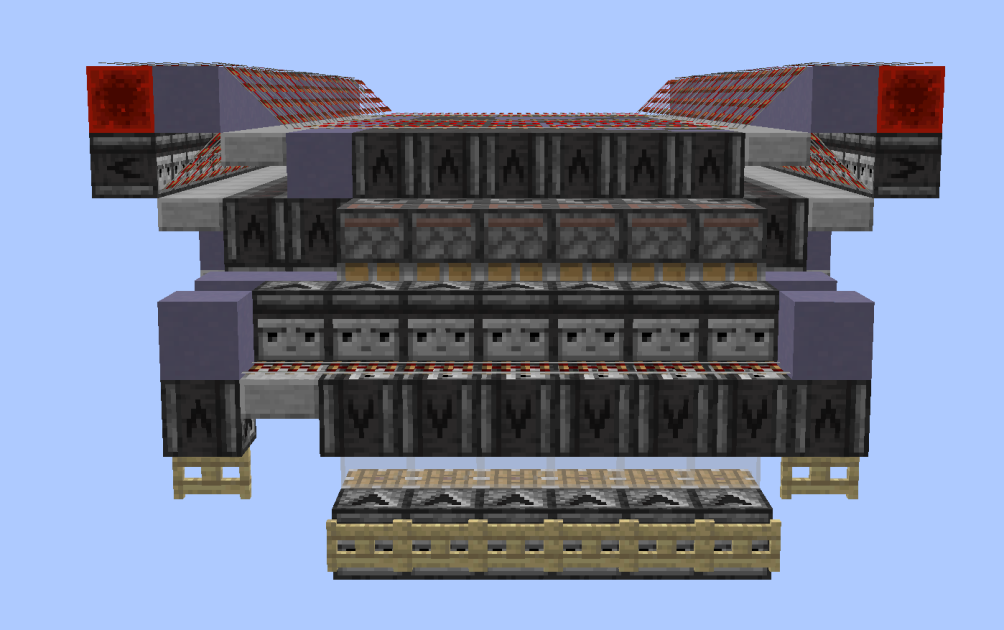
\includegraphics[width=0.48\textwidth]{dualdecoder.png}
    \caption{\centering Dual Sided 6 Bit Binary Decoder}
\end{figure}

% For wide tables, a single column layout is better. It can be switched
% page-by-page.
\onecolumn

\section{Device Specifications}

\begin{table}[h]
    \caption{Inputs}
    \begin{tabularx}{\textwidth}{l | c | X}
        \thickhline
        \textbf{Name} & \textbf{Range} & \textbf{Description} \\
        \hline
        Bits 1-6 & 0-1 & Binary input \\
        \hline
        Execute Left & Pulse & Clock signal of device. Outputs to left side of the device. \\
        \hline
        Execute Right & Pulse & Clock signal of device. Outputs to right side of the device. \\
        \thickhline
\end{tabularx}
\end{table}

\begin{table}[h]
    \caption{Outputs}
    \begin{tabularx}{\textwidth}{l | c | X}
        \thickhline
        \textbf{Name} & \textbf{Range} & \textbf{Description} \\
        \hline
        Mapped signal left & Pulse & Outputs to one of 64 slices corresponding to input code on the left side of the decoder. \\
        \hline
        Mapped signal right & Pulse & Outputs to one of 64 slices corresponding to input code on the right side of the decoder. \\
        \thickhline
\end{tabularx}
\end{table}

\begin{table}[h]
    \caption{Device Specifications}
    \begin{tabularx}{\textwidth}{l | c c c | c | X}
        \thickhline
        \textbf{Parameter} & \textbf{Min.} & \textbf{Typ.} & \textbf{Max.} &
        \textbf{Unit} & \textbf{Conditions} \\
        \hline
        Throughput  & 8 & - & - & gt & Normal Usage \\
        \hline
        Latency  & 12 & - & - & gt & Input to Output. \\
        \hline
        Active Lag & +3.4 & +3.5 & +3.6 & ms & At Hopperspeed. Ryzen 5 3600, 2GB RAM. MC 1.19.3 with Lithium. \\
        \hline
        MC Version & 1.11 & 1.19.3 & - & MCV & Latest version at time of writing: 1.20.4\\
        \hline
        Dimensions & & 68 x 8 x 13 & & Blocks & \\
        \thickhline
\end{tabularx}
\end{table}
\newpage
\section{Testing Data}
\begin{table}[h]
\caption{Executed Tests}
\begin{tabularx}{\textwidth}{l | X}
    \thickhline
    \textbf{Test} & \textbf{Result} \\
    \hline
    Code test & Device was able to decode all possible codes successfully.\\
    \hline
    Throughput test & Device was able to decode at 8gt throughput.\\
    \thickhline
\end{tabularx}
\end{table}

\section{Download Information}
\begin{table}[h]
    \caption{Download Information}
    \begin{tabularx}{\textwidth}{l | l | l | X}
        \thickhline
        \textbf{Identifier} & \textbf{MC} & \textbf{File} & \textbf{Description} \\
        \hline
        DC04 & 1.17 & \href{https://github.com/Soontech-Annals/Archive/blob/63c9ea8c34519ca4eb58649773e0c37e7e462fdd/Archive/decoders/DC04\%20Dual\%20Sided\%206\%20Bit\%20Binary\%20Decoder/DC04\_Dual\_Sided\_6\_Bit\_Binary\_Decoder\_1.17.litematic?raw=1}{DC04\_Dual\_Sided\_6\_Bit\_Binary\_Decoder\_1.17.litematic} & Litematic of decoder. \\
        \hline
        \thickhline
    \end{tabularx}
\end{table}

\end{document}

